\documentclass[tikz]{standalone}

\usepackage{fontspec}
\setmainfont[Ligatures=TeX, Mapping=tex-text]{Lato}
\usepackage{tikz}
\usetikzlibrary{arrows.meta}
\usepackage{xfp}

\begin{document}
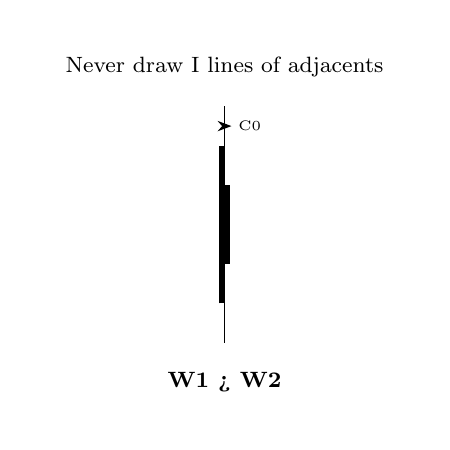
\begin{tikzpicture}

\def\width{5}
\def\height{5}
\def\ox{\fpeval{\width /2}}
\def\oy{\fpeval{\height /2}}

\tiny
\path [use as bounding box] (0,0) rectangle (\width,\height);

% PORTS
\draw [line width=2pt] (\ox,\oy) ++(-1pt,0) +(0,-1) -- +(0,1);
\draw [line width=2pt] (\ox,\oy) ++(1pt,0) +(0,-0.5) -- +(0,0.5);

% MESH
\draw [line width=0.5pt] (\ox,\oy) +(0,-1.5) -- +(0,1.5);
\path [tips, -{Stealth[length=5pt]}](\ox,\oy) ++(0,1.25) -- +(2.5pt,0) node[right] {C0};

% CONDITION
\draw (\ox,\oy) ++(0,-2) node {\footnotesize\textbf{W1 > W2}};

% NOTE
\draw (\ox,\oy) ++(0,2) node {\footnotesize Never draw I lines of adjacents};

\end{tikzpicture}
\begin{tikzpicture}

\def\width{5}
\def\height{5}
\def\ox{\fpeval{\width /2}}
\def\oy{\fpeval{\height /2}}

\tiny
\path [use as bounding box] (0,0) rectangle (\width,\height);

% PORTS
\draw [line width=2pt] (\ox,\oy) ++(1pt,0) +(0,-1) -- +(0,1);
\draw [line width=2pt] (\ox,\oy) ++(-1pt,0) +(0,-0.5) -- +(0,0.5);

% MESH
\draw [line width=0.5pt] (\ox,\oy) +(0,-1.5) -- +(0,1.5);
\path [tips, -{Stealth[length=5pt]}](\ox,\oy) ++(0,1.25) -- +(-2.5pt,0) node[left] {C0};

% CONDITION
\draw (\ox,\oy) ++(0,-2) node {\footnotesize\textbf{W1 < W2}};

% NOTE
\draw (\ox,\oy) ++(0,2) node {\footnotesize Never draw I lines of adjacents};

\end{tikzpicture}
\begin{tikzpicture}

\def\width{5}
\def\height{5}
\def\ox{\fpeval{\width /2}}
\def\oy{\fpeval{\height /2}}

\tiny
\path [use as bounding box] (0,0) rectangle (\width,\height);

% PORTS
\draw [line width=2pt] (\ox,\oy) ++(-0.5pt,0) +(0,-0.5) -- +(0,0.5);
\draw [line width=2pt] (\ox,\oy) ++(0.5pt,0) +(0,-0.5) -- +(0,0.5);

% CONDITION
\draw (\ox,\oy) ++(0,-2) node {\footnotesize\textbf{W1 == W2}};

% NOTE
\draw (\ox,\oy) ++(0,2) node {\footnotesize Never draw I lines of adjacents};

\end{tikzpicture}
\end{document}
